%%%%%%%%%%%%%%%%%%%%%%%%%%%%%%%%%%%%%%%%%%%
%%% DOCUMENT PREAMBLE %%%
\documentclass[12pt]{report}
\usepackage[english]{babel}
%\usepackage{natbib}
\usepackage{url}
\usepackage[utf8x]{inputenc}
\usepackage{amsmath}
\usepackage{graphicx}
\graphicspath{{images/}}
\usepackage{parskip}
\usepackage{fancyhdr}
\usepackage{vmargin}
\usepackage[T1]{fontenc} % Use 8-bit encoding that has 256 glyphs
\usepackage{booktabs} % for nice lines in tables
\usepackage{color} % text color
\setmarginsrb{3 cm}{2.5 cm}{3 cm}{2.5 cm}{1 cm}{1.5 cm}{1 cm}{1.5 cm}

\title{Applying Reinforcement Learning to Bomberman}								
% Title
\author{Hein-Erik Schnell, Karl Thyssen}						
% Author
\date{\today}
% Date

\makeatletter
\let\thetitle\@title
\let\theauthor\@author
\let\thedate\@date
\makeatother

\pagestyle{fancy}
\fancyhf{}
\rhead{\theauthor}
\lhead{\thetitle}
\cfoot{\thepage}

% displays code within text
\newcommand{\code}[1]{{\fontfamily{pcr}\selectfont #1}}
\newcommand{\state}[1]{$\left\lbrace #1 \right\rbrace$}

% Define command \chapterauthor{author}
\makeatletter
\newcommand{\chapterauthor}[1]{%
	{\parindent0pt\vspace*{-10pt}% Vspace btw heading and author
		\linespread{1.1}\itshape#1 % \itshape is text formatting (italic) 
		\par\nobreak\vspace*{10pt}} % Vspace btw author and text
	\@afterheading%
}
\makeatother


%%%%%%%%%%%%%%%%%%%%%%%%%%%%%%%%%%%%%%%%%%%%
\begin{document}

%%%%%%%%%%%%%%%%%%%%%%%%%%%%%%%%%%%%%%%%%%%%%%%%%%%%%%%%%%%%%%%%%%%%%%%%%%%%%%%%%%%%%%%%%

\begin{titlepage}
	\centering
    \vspace*{0.5 cm}
    
\includegraphics[scale = 0.075]{uni_hd_logo.jpg}\\[1.0 cm]	% University Logo
\begin{center}    \textsc{\Large   Fundamentals of Machine Learning}\\[2.0 cm]	\end{center}% University Name
	\textsc{\Large Final Project  }\\[0.5 cm]				% Course Code
	\rule{\linewidth}{0.2 mm} \\[0.4 cm]
	{ \huge \bfseries \thetitle}\\
	\rule{\linewidth}{0.2 mm} \\[1.5 cm]
	
	\begin{minipage}{0.4\textwidth}
		\begin{flushleft} \large
		%	\emph{Submitted To:}\\
		%	Name\\
          % Affiliation\\
           %contact info\\
			\end{flushleft}
			\end{minipage}~
			\begin{minipage}{0.4\textwidth}
            
			\begin{flushright} \large
			\emph{Submitted By :} \\
			Hein-Erik Schnell\\
			Karl Thyssen  
		\end{flushright}
           
	\end{minipage}\\[2 cm]
	
	%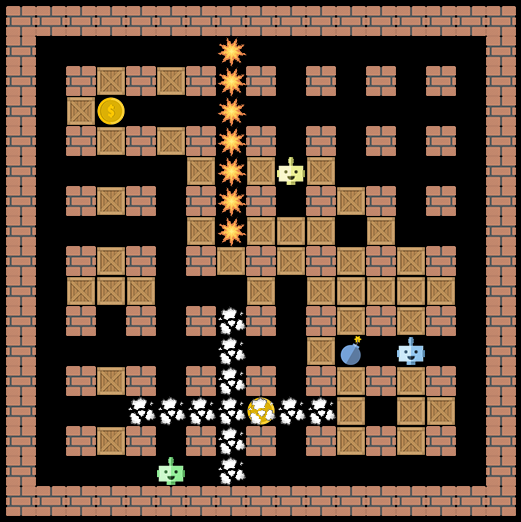
\includegraphics[scale = 0.3]{Bomberman_title.png}
    
    \code{https://github.com/nessyht/FOML-Bomberman}
    
\end{titlepage}

%%%%%%%%%%%%%%%%%%%%%%%%%%%%%%%%%%%%%%%%%%%%%%%%%%%%%%%%%%%%%%%%%%%%%%%%%%%%%%%%%%%%%%%%%

\tableofcontents
\pagebreak

%%%%%%%%%%%%%%%%%%%%%%%%%%%%%%%%%%%%%%%%%%%%%%%%%%%%%%%%%%%%%%%%%%%%%%%%%%%%%%%%%%%%%%%%%
\renewcommand{\thesection}{\arabic{section}}

\section{Learning Method and Regression Model}
\chapterauthor{Hein-Erik Schnell}
This section is divided into the three crucial tasks for which we needed to develop a concept in order to get the agent into training. Those tasks were:

\begin{itemize}
	\item Choosing a suitable \textit{state representation} to be then passed to an \textit{regressor} to estimate the expected \textit{reward} for each of the possible actions
	\item Choosing suitable \textit{rewards} in order to communicate the goals of the game to the agent
	\item Choosing a suitable \textit{regressor} which estimates the expected \textit{reward} for each possible action at the current state of the game.
\end{itemize}

	\subsection{State representation}
	\chapterauthor{Hein-Erik Schnell}
	The first task was to choose a suitable state representation. In case of regressors provided by \textit{scikit-learn}, the training data is usually passed to the regressor as a 2D-array where each row (first index) represents a single state and each column (second index) represents a feature of the respective states. Analagously, the prediction then demands an array of similar form. The regressor then returns an array with as many predicted values as there were rows (states) in the input array. If one wants to predict only a single value, one may not pass a 1D-array to the regressor but create an additional dummy dimension. All this means that if we want to use precoded regressors from scikit-learn, we need to find a 1D-array representation for a single state. \par
	
	After each step, the relevant data is passed to the agent via the dictionary \code{self.game\_state}. In the agents \code{callbacks.py} we defined the function \code{create\_state\_vector(\textit{self})} which turns the information provided by \code{self.game\_state} into a 1D-array. We chose to store the relevant features in the following way:
	
	\subsubsection{State representation 1}
	\label{State_rep_1}
	\begin{itemize}
		\item For each cell:
		\begin{itemize}
			\item \textbf{Agent, Opponent, None \state{1,-1,0}}:\\
			The dictionary provides the entry \code{self.game\_state['arena']} which is a 2D representation of the game board. We use this to create a numpy-array \code{agent\_state} of the same shape which is $1$ on the agents position, $-1$ on cells with an opponent and $0$ on all other cells.
			\item \textbf{Crate, Coin, Empty/Wall \state{-1,1,0}}: \\
			A copy of \code{self.game\_state['arena']} is manipulated in such a way that it is $-1$ for a crate, $1$ for a coin on the respective cell and $0$ in all other cases. This would mean that the agent could not distinguish between empty cells and walls. This issue is resolved later when we delete all cells which contain walls. These cells are always the same and therefore do not contribute to the learning process. In our code, this whole part is represented by the variable \code{loot\_state}.
			\item \textbf{Bombs} \state{6,5 \dots 2,1,0}:\\
			The variable \code{bomb\_state} is of the same shape as \code{self.game\_state['arena']}. All cells are by default $6$. If the cell will soon be affected by a bombs explosion, the values $5\dots2$ represent the 4-time-steps countdown. $1\dots0$ represent the 2-time-steps explosion. This way, \code{bomb\_state} provides a danger level for each cell. $6$ means no danger at all.
			
		\end{itemize}
		\item Just once (implemented in our code as \code{extras}):
		\begin{itemize}
			\item \textbf{Current step number \state{1,\dots,400}}:\\
			\code{extras[0]} contains the current time step.
			\item \textbf{Danger level} \state{0,\dots,6}:\\
			\code{extras[1]} represents the danger level on the agents current position. It is calculated by $6 - \text{\code{bomb\_state[x,y]}}$, where \code{x} and \code{y} are the coordinates of the agents position. Consequently, this danger level in invers to the danger level in \code{bomb\_state}, i.e. $0$ means no danger, $1\dots4$ means increasing danger and $5\dots6$ would be bombs exploding. The least point is rather irrelevant since the agent would already have been deleted by the environment.
			\item \textbf{Bomb action possible \state{0,1}}:\\
			\code{extras[2]} is $1$ if the agent could place a bomb and $0$ if not (i.e. if an own bomb is still ticking).
			\item \textbf{Touching opponent} \state{0,1}:\\
			\code{extras[3]} is $1$ if an opponent is on a neighbouring cell and $0$ if not.
		\end{itemize}
	\end{itemize}

	After manipulating the data in the described way, all cells containing walls are deleted from the 2D-arrays \code{agent\_state}, \code{loot\_state} and \code{bomb\_state}. As already described above, this is done because these entries will always be the same and therefore never contribute to the learning of the agent. The three arrays are then flattened and concatenated after one another into the 1D-array \code{vector}. Finally, we append the \code{extras} to the \code{vector}, which is then returned by the function \code{create\_state\_vector}.\par
	
	With the described representation of a state we combined features which could be represented as seperate features into single features. For example in \cite{paper}, each cell has a feature \textit{Agent on cell?} and \textit{Opponent on cell?} which can both assume the values $0$ and $1$. We combined these two features. As we see it, a proper regressor should be able to determine the important features as well as the relevant range of values of a feature. A \textit{Random Forest Regressor}, for instance, should theoretically be able to do so since the way it works is to find the most relevant feature and its most divisive value.\par
	
	With \textit{state representation 1} ($532$ features), the feature space has at most about $5.4 \times 10^{320}$ possible states. 
	% Calculated with 3^(17*17-34-30-49) * 3^(17*17-34-30-49) * 7^(17*17-34-30-49)*400*7*2*2
	
	\subsubsection{State representation 2}
	\label{State_rep_2}
	As described later in section \ref{results}, our agent never managed to get out of its starting corner. In order to change that, we condensed the above state vector ($532$ features) into a much smaller state vector of $180$ features. The main idea of this smaller state vector is that agents, opponents, crates and coins can never occupy the same cell. Bombs could occupy the same cell as agents, opponents or coins, but for the sake of the agent they shouldn't:
	
	\begin{itemize}
		\item For each cell:
		\begin{itemize}
			\item \textbf{Empty, agent, opponent, crate, coin, danger level} \state{0,1,2,3,4,5 \dots 11}:\\
			Empty cells are $0$. Cells with agent, opponent, crate or coin are \state{1,2,3,4}, respectively. The values \state{5 \dots 11} represent the danger level because there is a bomb affecting the respective cell. $5$ is not used, \state{6 \dots 9} is the four-time-steps countdown, \state{10,11} the two-time-steps explosion. If there is a danger level the values \state{1,2,3,4} are overwritten. This means that the position of the agent might not be represented anymore in this feature.
		\end{itemize}
		\item Just once (implemented in our code as \code{extras})
		\begin{itemize}
			\item \textbf{Danger level} \state{6 \dots 11}:\\ 
			\code{extras[0]} is the danger level at the position of the agent.
			\item \textbf{Bomb action possible} \state{0,1}: \\
			\code{extras[1]} is $1$ if the agent could place a bomb and $0$ if not (i.e. if an own bomb is still ticking).
			\item \textbf{Touching opponent} \state{0,1}: \\
			\code{extras[2]} is $1$ if an opponent is on a neighbouring cell and $0$ if not.
			\item \textbf{Position of agent} \state{18 \dots 271}: \\
			\code{extras[3]} is essentially the enumerated cell number of the agents position. It is calculated by $17x + y$, where $x$ and $y$ are the agents $x$- and $y$-coordinates. 
		\end{itemize} 
	\end{itemize}
	
	With \textit{state representation 2} (180 features) it has at most about $3.4 \times 10^{193}$ possible states, which is much less than with \textit{state representation 1}. For both representations, these are only upper limits. But both are calculated the same way so that these values are useful for comparisons between both representations.
	% Calculated with 12^(17*17-34-30-49) * 6 * 2 * 2 * (17*17-34-30-49)
	
	\subsection{Rewards}
	\chapterauthor{Karl Thyssen}
	The individual rewards for events that occur in a given step contribute to the reward function and are explicitly defined in the \code{reward\_update()} and \code{end\_of\_episode} functions. The other parameter to influence is the discount factor $\gamma$ for the discounted long term reward. We ran training with factors $\gamma = 1.0$ and $\gamma = 0.9$. The reward function is described by a series of \code{if} clauses that determine the quality of the action taken and apply the reward.

\begin{itemize}
	\item \textbf{Valid move}: $-1$ \\Every step is punished in a small way to encourage the agent to complete tasks in the shortest possible time to avoid stacking negative rewards.
	\item \textbf{Wait}: $-5$\\We noticed while running preliminary quick trains that the agent quickly regressed into a pattern of repeated 'Wait's after only a few generations. Arguably other factors were also different at the time so its debatable how effective this now is.
	\item \textbf{Invalid action}: $-100$\\Invalid actions should be punished so the agent quickly learns the connections in between the fields and the restrictions on the frequency of bomb placements.
	\item \textbf{Destroy crate}: $+10$\\The agent should learn to destroy crates.
	\item \textbf{Coin found}: $+20$\\The agent should want to destroy as many crates as possible to find coins.
	\item \textbf{Collect coin}: $+2000$\\The agent is heavily rewarded for finding coins to incentivise coin collection as a primary goal.
	\item \textbf{Killed opponent}: $+10000$\\If the agent does accidentally kill an agent in training it should have a large weighting so this behaviour can be encouraged, particularly as this will be rare initially.
	\item \textbf{Die (from opponent bomb)}: $-2000$\\The agent should learn to avoid all bombs \dots
	\item \textbf{Die (suicide)}: $-1500$\\ \dots but rather die to its own to deny opponents 5 points.
\end{itemize}	
	
	We did not change the rewards in our tweaking due to the fact that we were not sure how to effectively test changes. Our superficial tests (anecdotal) never lead to ground breaking changes and as such we couldn't realistically change them with the expectation that something would be positively influenced. Particularly reflecting the amount of time it would have taken to train even 10 generations of the changes. However, some interesting ideas we would perhaps have next investigated are:
	\begin{itemize}
		\item Whether a movement to a cell should be rewarded based on proximity to other agents/bombs or coins and how we allow these factors to influence the positivity or negativity of an action. I.e. a step towards a coin that is also a step into an exploding bomb should lead to a negative reward.
		\item Should we punish the repetition of actions, such as the movement to a previously occupied cell which may be undesirable and therefore punished with a small negative value, or should this only be the case when not running from a bomb?
		\item Not punishing death or any actions we perceive to be negative but rather only enforce good ones and let the agent decide whether the risks are worth taking that is to say whether the punishment of not getting the reward is discouragement enough.
	\end{itemize}
	
	\subsection{Regressors}
	\chapterauthor{Hein-Erik Schnell}
	In order to estimate the expected rewards properly we need to find a regressor which is both flexible and very decisive with respect to the features. Flexible, because a simple linear regressor would not be able to resemble the volume of states and outcomes. This big variety of possible states, even at the very beginning of an episode, means that many features are not relevant in a given situation. This is the reason why the regressor should also be able to find the most decisive features.\par
	
	Since we will not know whether the competition will be split into two leagues, one for neural networks and one for classical regressors, we initially decided to train both a classical regressor and a neural network and see which one performs better (in its respective league).\par
	
	As a classical model we chose to use a \textit{Random Forest Regressor}. The advantage of this regressor is that it is infinitely flexible can and can cope with whatever shape the reward function may assume. However, it turns out that this regressor is also quite inaccurate and erratic. Its erratic nature might be problematic because the order of the estimated rewards, i.e. which move is the best, is very important. If the order can not be predicted correctly the agent will not choose the best but only a good move. Figure \ref{forest_mlp_comp2} shows how likely this is. We chose to use the Random Forest Regressor provided by \textit{scikit-learn}.\par
	
	As a neural network we chose the \textit{MLP-Regressor} provided by \textit{scikit-learn} mainly for two reasons. The first reason is that we need a precoded regressor since neural networks haven't been subject to the lecture yet. The other reason is that the syntax and available functions of that regressor are the same as for the Random Forest Regressor. This way we only need to change the initialization of our regressor and do not have to change the rest of the code. It is basically changing one line of the code in order to switch between both regressors.\par
	
	The two regressors are initialized as follows:
	\begin{itemize}
		\item \code{RandomForestRegressor()}
		\item \code{MLPRegressor(max\_iter=500)}
	\end{itemize}
	Thus, we used the Forest with its default settings and changed the maximum number of iterations of the MLP to $500$ (default is $200$) because the regressor sent out a warning that $200$ iterations were not sufficient to reach convergence.
	
	\begin{figure}[h]
		\centering
		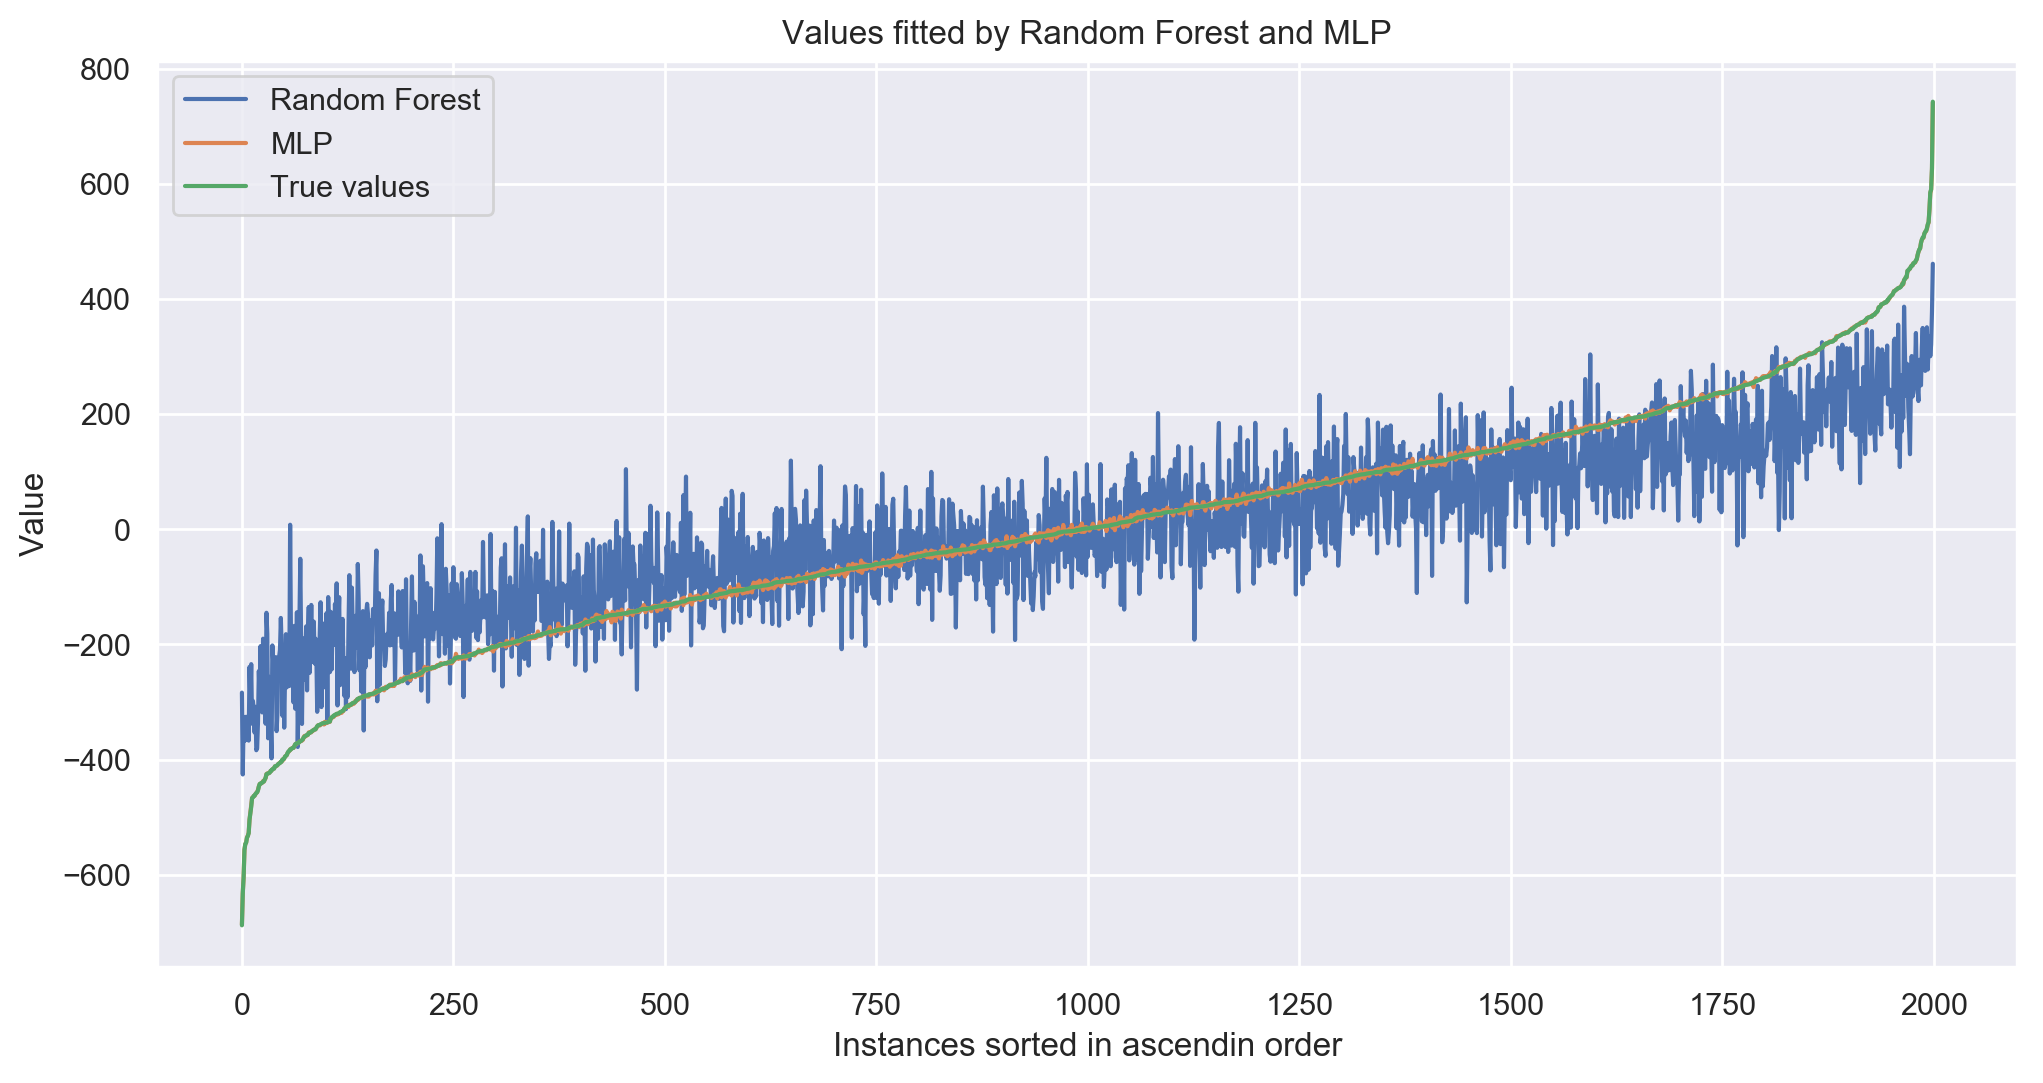
\includegraphics[width=\linewidth]{images/mlp_forest_comparison01.png}
		\caption{\textit{For this figure, {\normalfont \code{sklearn.datasets.make\_regression}} was used to create $10000$ samples with $100$ features of which $10$ are informative. We then trained the Random Forest Regressor and the MLP-Regressor provided by {\normalfont scikit-learn} with $80\%$ of the generated data. The figure shows the predicted values of the remaining $20\%$ of the data which were used as a test set. The test set has previously been sorted by the true target value in ascending order.}}
		\label{forest_mlp_comp1}
	\end{figure}
	\begin{figure}[h]
		\centering
		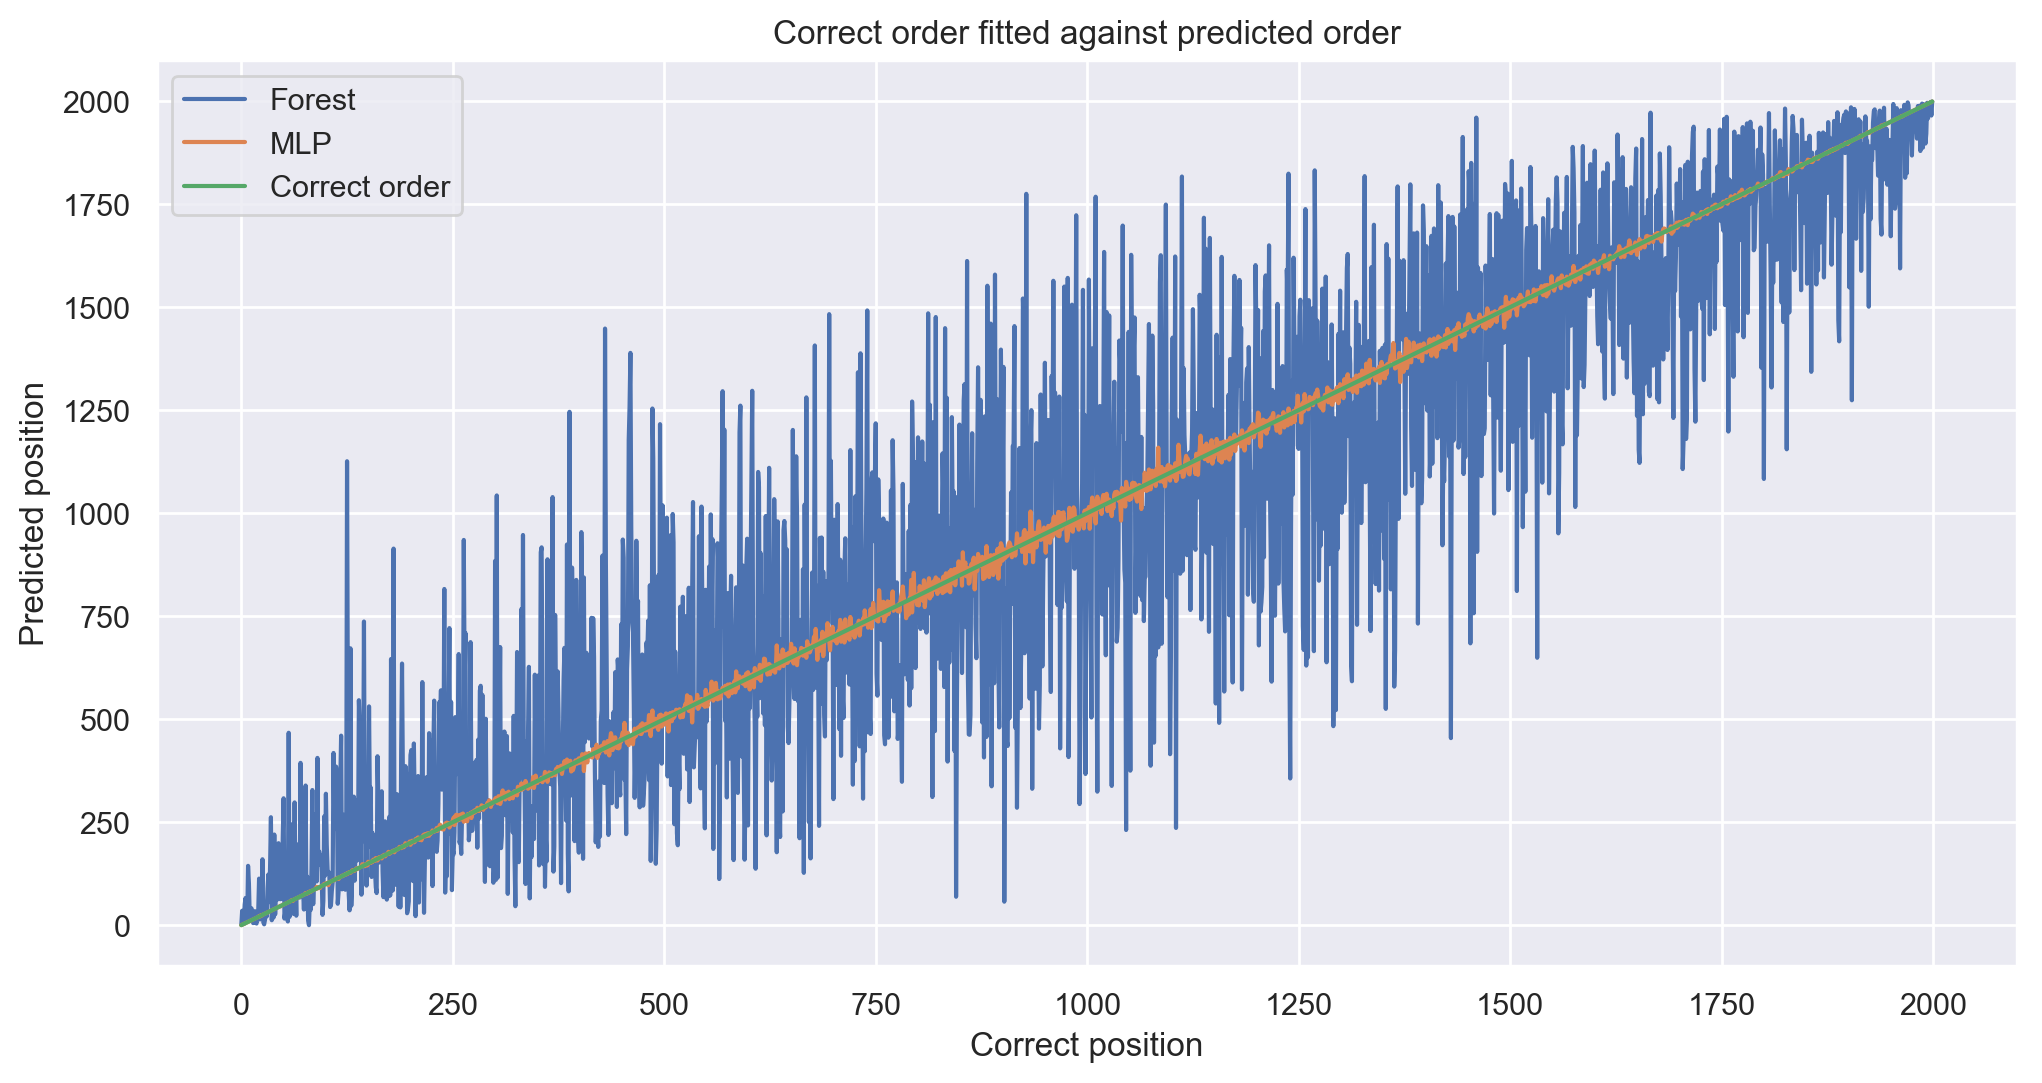
\includegraphics[width=\linewidth]{images/mlp_forest_comparison02.png}
		\caption{\textit{This figure displays the same data as Figure 1. Here, the x-axis represents the position of each instance sorted by its target value, the y-axis displays the position if the instances had been sorted by the predicted target values of the respective regressor. The more the predictions resemble the correct order (the green line) the better the regressor is suited for our task.}}
		\label{forest_mlp_comp2}
	\end{figure}

	In order to get a feeling for the performance of both regressors, we used the function \code{sklearn.datasets.make\_regression} to create $10000$ samples with $100$ features of which $10$ are informative. We then trained the Random Forest Regressor and the MLP-Regressor with $80\%$ of the generated data and let both regressors predict the values of the remaining $20\%$ of the data. Figure \ref{forest_mlp_comp1} shows how much more accurate the MLP-regressor performs compared to the Random Forest Regressor. Figure \ref{forest_mlp_comp2} shows how the MLP-Regressor maintains the order of the instances much better than the Random Forest Regressor. In case of the latter, many values are sorted into completely other regions than where they actually belong. This is also due to the fact that the range of values of the generated data is of the same magnitude as the inaccuracies of the Forest. Still, the MLP manages to predict these values much better.
\newpage
	
	
\section{Training Process}
\chapterauthor{Karl Thyssen}
In reinforcement learning an agent is placed into an environment where it learns to interact with it dependent on the parameters a 'trainer' provides it. Ideally the trainer wishes the agent to embody certain desirable characteristics. This optimal policy is determined by the methodology the trainer uses to reward the agent. Rewards the trainer supplies the agent with are based on the state of the environment at the time the agent is to make a decision and the reward scheme weighting on this given state. 

Initially the agent is often allowed to take random actions to influence the next game-state. This random acting forms the agents initial policy $\pi$. The policy determines how the agent acts in the game, the ideal policy being the ideal way to play the game from the initial game-state.

The rewarding of an agent for a particular action $a$, functions to provide information as to the quality of the decision it made to take this particular action at this particular state $s$; this \state{(state, action)} pair $(s, a)$. Through this feedback the agent can update its policy. Through regular updates of the policy($\pi$), after receiving a reward for games played based on the current policy the agent will begin to favour actions it predicts will lead to higher rewards hence improve the policy and bring it as closely as possible to the optimum.

Formally this is known as the Markov-Decision-Process where the state of the environment at a particular step $t$ in the game is represented as $s_t$ and the action taken for this time step t is represented as $a_t$. The current state is input into the current policy which leads the agent to select its next action. The action is selected from the action space $\mathcal{A} = $\state{\text{UP}, \text{LEFT}, \text{DOWN}, \text{RIGHT}, \text{BOMB}, \text{WAIT}}. The reward for this action $r_t$ is then given by the reward function $r(s_t, a_t)$ given which the agent can then evaluate this move for the update of its policy. In Bomberman its simple to see that the state $s_t$ is given by the distribution of agents, loot, bombs, coins etc. in the game map represented as the trainer wishes. 

In Bomberman an action can not be rewarded entirely isolated from the game as a whole as actions have direct repercussions least 6 steps into the future (by the time the explosion has dissipated) and even beyond. Therefore the action must be rewarded based on all future steps with those very far in the future having decreasing impact. Therefore we introduce a discount factor $\gamma \in [0, 1]$. We arbitrarily selected 0.9 to ensure the steps $n+4, n+5, n+6$ have a non-negligible impact on the reward, as these are the steps that we hope to cash in from a bomb and the agent should see that this was a well placed bomb if this is the case. Unfortunately we see this being very negative as the agent often self-destructs...

Therefore the reward function that the agent is wishing to maximise the expected long term reward $E[\text{Reward}|\pi]$ for the optimal policy is: $$\text{Reward} = \sum_{t=0}^{\infty} \gamma^t r_{t+1}$$. 

The concept of learning refers to the improvement of this policy, by two processes, policy improvement and policy evaluation. As the initial policy in our case will be created by either the random actions of the \code{random\_agent} or the deterministic actions of the \code{simple\_agent}, the initial policy evaluation step will take place on this gathered data.  This is achieved using a value function for each of the states visited in this policy $\pi$. The value function $V$ for each state $s_t$ is the Expected value given the starting state is $s$ of the discounted reward function of the $\pi(a_t|s_t)$ particular pair.

	\subsection{Q-Learning}
	\chapterauthor{Karl Thyssen}
	With our selected state vector of length 532 it would be highly impractical of not impossible to calculate the state action pairs for every state and the expected reward of each action due to the massive amount of data required for this along with the computationally intensive time requirement. Therefore we use the approach of Q-Learning to find the optimal Q function $Q^*$ for each state-action pair in the data, updated using the discounted reward received for the action. We do this in the callback function of the agent when \code{end\_of\_episode()} is called, the discounted rewards are filled into the places of the previously stored immediate rewards of each state-action pair. 
	
	This Q function will need to be updated to find the optimal Q function by gathering data, evaluating the data and updating. To gather data we have 3 options: update Q after every step, after every n-steps or after every n-episodes. Due to the fact that we selected random forest regressors to store our Q the last option seems to suit the purpose best as it is not possible to update sklearn random forest regressors, they must rather be entirely trained from scratch. Therefore it would be incredibly time and storage inefficient to train them on multiple steps, particularly as they will not be effective with small data pools anyway. Therefore we opt to update Q after 10000 as suggested in \cite{paper}.
	
	We store our Q-function as 6 random forest regressors; one for each action, from which the agent will choose an action based on the stochastic policy of the trained forests, each supplying the expected reward for the action it is trained for. This action $a_{t+1} = \pi(a_t|s_t)$ will, in training, be mapped onto the calculated reward along with all state action pairs in the 10,000 games played during each particular policy iteration to retrain the forests, that is to say update the Q-function.
	
	
	\subsection{Exploration and exploitation}
	\label{explo}
	\chapterauthor{Hein-Erik Schnell, Karl Thyssen}
	While optimising the Q function based solely (exploitative approach) on the games of the previous generation (the trees trained on the past $10,000$ games) it is possible to slip into a local maximum in terms of the yield which may well not be the optimal Q. Therefore we introduced a degree of exploration using an $\epsilon$-greedy policy in which a random action is performed with the probability $\epsilon \in [0,1]$. We selected $\epsilon = 0.25$. \par
	
	\subsubsection{Max-Boltzman-exploration}
	When exploration occurs (not the best action is chosen), we decided not to choose the action completely random. Instead, choosing more promising actions should be more likely. This means that the expected rewards need to be mapped onto probabilities with which the respective action is chosen. The probability is given by 
	\begin{align}
		\pi (s,a) = \frac{e^{Q(s,a)/T}}{\sum_{a} e^{Q(s,a)/T}}\text{,}
	\end{align}
	where $\pi (s,a)$ is the probability that the action $a$ is chosen given state $s$, $Q(s,a)$ is the expected reward if action a is performed after state $s$ occured, $a \in \mathcal{A}\setminus a_{max}$ are all available actions after the action with the highest expected reward $a_{max}$ has been deleted from the set of actions $\mathcal{A}$ because $a_{max}$ would have been chosen if we didn't explore, and $T$ is a temperature-parameter which scales the ratios between the probabilities. We found that $T$ should be of about the same magnitude as the expected rewards which is why we chose $T$ as the mean of the absolute values of the expected rewards. Figure \ref{MB_table} shows an example of this.
	\begin{figure}[h]
		\centering
		\begin{tabular}{c|c}
			$Q(s,a)$ & $\pi (s,a)$\\
			\midrule
			$43$ & $0.52$\\
			$21$ & $0.25$\\
			$4$ & $0.14$\\
			$-19$ & $0.07$\\
			$-65$ & $0.02$
		\end{tabular}
	\caption{\textit{Exemplary table of expected rewards $Q(s,a)$ and corresponding probabilities $\pi (s,a)$ if $T$ is chosen as described above. In this case: $T=30.4$}}
	\label{MB_table}
	\end{figure}
	We later decided to enable \textit{exploration} only in one fourth of all rounds. The reason is that the agent can only survive after it placed a bomb if it moves consistently away from it or around a corner. Thus, a random move in every fourth step may be fatal. With the above measure, we could at least ensure the survival after placing a bomb and make the agent learn this behaviour.
	
	\subsection{Training data}
	\chapterauthor{Karl Thyssen}
	We generated new training data after each training generation of $10,000$ games to train the new forests that is to say the Q function for the next generation to learn from. Therefore the size of our final training data array of action state vectors was dependent on the number of rounds the agent survived in a given generation. We saved each set of training data independently of each other to allow for training from any generation and later access to the data. The random forest regressors were also saved to allow for analysis of them and comparison between the generations by allowing play from any generation and even play against younger generation. Ideally play against younger generations would always lead to free wins as the agent should be significantly better after some time, however our agent is a lonely agent that rarely sees others anywhere other than in its state vectors.


\section{Results}
\label{results}
\chapterauthor{Karl Thyssen}
Here we will discuss the results we saw for the various approaches we attempted.

As previously mentioned we experimented with a $\gamma$ value of $1.0$ and $0.9$ after which we continued other variations at $\gamma = 0.9$.
Other variations include:
\begin{itemize}
	\item $\gamma = 1.0$:
	\begin{itemize}
		\item Generation 0 data generated from 4 $\code{simple\_agents}$
		\begin{itemize}
			\item Additionally train MLB
		\end{itemize}
	\end{itemize}
	\item $\gamma = 0.9$:
	\begin{itemize}
		\item Generation 0 data generated from 4 $\code{simple\_agents}$:
		\begin{itemize}
			\item self-train until agents begin to regularly interact with each other
			\item self-train
			\item state vector reduced to 180 elements
		\end{itemize}
		\item Generation 0 data generated from 4 $\code{random\_agents}$:
		\begin{itemize}
			\item self-train until agents begin to regularly interact with each other
			\item self-train
		\end{itemize}
	\end{itemize}
\end{itemize}

%Discuss reasons behind initial approach - also mlp regressor (slow to fit so less data)
\subsection{The initial approach}

Having decided on the random forest regressors as the medium for storing our Q, and knowing the random forest has the ability to determine feature importances and weightings itself we decided to throw every feature we could think at it as described in \ref{State_rep}. We initially also chose a $\gamma$ value of $1.0$ for simplicity in testing and began to train an agent. In \cite{paper} the agent trains for 10000 episodes per generation and begins to show a large improvement between generations $10$ and $20$, however that agent is trained using a neural network so we expected a longer wait before seeing such spikes in performance. This is due to the erratic nature of the predictions made by the forests in relation to the MLP we tested.

Out of interest we also tested the same set-up using an MLP regressor, however unlike the forest, the impact of using any and all features was an exorbitant time required for the fitting after each generation, often longer than the data generation itself.

The average time required to generate data for and fit each generation was roughly $4800 seconds$. This time required is clearly dependent not only on hardware and thinking time but also the number of steps the agent takes per episode which was unfortunately consistently short.

\begin{figure}[h]
\centering
	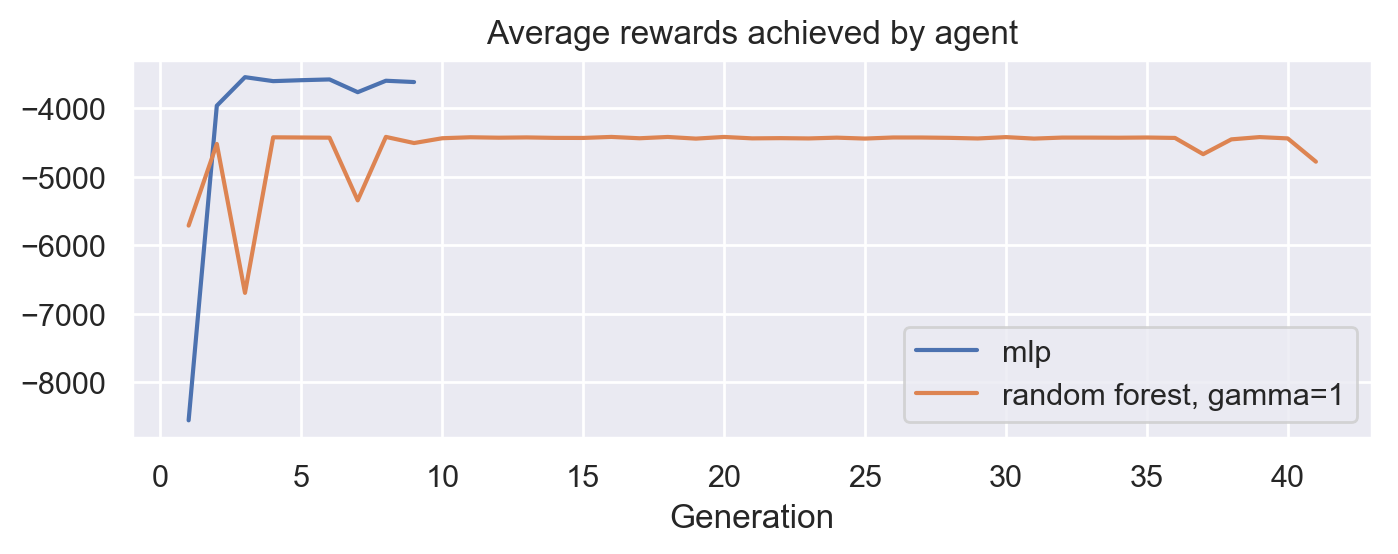
\includegraphics[width=\linewidth]{images/mlp_vs_forest_gamma_1.png}
	\caption{Here we see the performance of 40 generations trained with the random forest and 8 generations using the MLP. We chose not to train the MLP further as the time constraints were too severe and we were not seeing any improvement.}
	\label{mlp_vs_forest_gamma_1.0}
\end{figure}


%show results of initial training
%random forest too erratic - as single steps can be fatal, inaccuracies can have drastic consequences
%let train for a long time as unclear when we should see results
%present variations
%discuss changes and possible solutions - even fewer features, other machine learning methods




%%%%%%%%%%%%%%%%%%%%%%%%%%%%%%%%%%%%%%%%%%%%%%%%%%%%%%%%%%%%%%%%%%%%%%%%%%%%%%%%%%%%%%%%%
\begin{thebibliography}{111}
   

%if the "underfill \hbox" warning bothers you uncomment the following line
%\raggedright


\bibitem{RL_intro}
Richard S. Sutton, Andrew G. Barto (2018)\\
\textit{Reinforcement Learning: An Introduction}\\
Available at: http://incompleteideas.net/book/bookdraft2018jan1.pdf

\bibitem{paper}
Joseph Groot Kormelink, Madalina M. Drugan and Marco A. Wiering (ICAART 2018)\\
\textit{Exploration Methods for Connectionist Q-Learning in Bomberman}\\
Available at: https://bit.ly/2GReSxQ
\end{thebibliography}
\end{document}

%This template was created by Roza Aceska.